\subsection{Application: Scientific Machine Learning for Climate and Weather Forecasting}

Weather forecasting is a useful Foundations application because it magnifies several machine-learning principles that are easy to overlook in static tabular benchmarks. The data are spatiotemporal fields rather than independent rows, validation must respect chronology, forecast errors accumulate during autoregressive rollout, and evaluation metrics must reflect the geometry of the Earth rather than treating every latitude-longitude grid cell as equally representative of surface area.

The application also demonstrates why headline accuracy is not sufficient for a scientific machine-learning system. A forecast can achieve a competitive aggregate RMSE while producing physically implausible small-scale structure, poor extreme-event skill, or unstable long-horizon rollouts. Reproducibility therefore requires exact benchmark versions, variables, pressure levels, forecast horizons, regridding choices, and evaluation code in addition to model architecture and optimizer settings.

The published benchmark context is WeatherBench/WeatherBench 2 and ERA5-based medium-range forecasting. The scientific figure used here is intentionally different: it is a reproducible Lorenz-96 simulation that isolates the core phenomenon of chaotic multivariate rollout. The simulation is used to teach temporal validation and error propagation; it is not presented as a substitute for ERA5 or as empirical evidence about operational weather skill.

\textbf{Problem}

The learning problem maps one or more atmospheric states to a future state and, for multi-step forecasts, recursively feeds predictions back into the model. This creates a distribution-shift problem inside the rollout itself: later predictions depend on earlier model errors. A defensible evaluation therefore reports performance as a function of lead time rather than only at one prediction step.

\textbf{Dataset}

Published weather benchmarks commonly use ERA5 reanalysis together with WeatherBench-style preprocessing and evaluation. The benchmark specification must identify the exact temporal range, spatial resolution, pressure levels, variables, initialization frequency, and evaluation period. The numerical figure in this section uses the Lorenz-96 dynamical system with 20 state variables and forcing parameter \(F=8\) as a compact chaotic surrogate for demonstrating rollout behavior.

\textbf{Model}

Modern published baselines include GraphCast, Pangu-Weather, FourCastNet, and operational numerical-weather-prediction systems. Their architectures differ substantially, so fair comparison requires matched data, variables, forecast horizon, and metric definitions. For the Chapter 1 treatment, the important distinction is not the architecture itself but the validation protocol used to compare learned and physics-based forecasts.

\textbf{Method}

Chronological partitions are required because random shuffling would leak future climate and seasonal structure into model selection. For a scalar field \(z\), latitude-weighted RMSE uses \(w_i=\cos(\phi_i)\) so that grid cells near the poles do not dominate merely because a regular latitude-longitude grid contains many cells there. Multi-step evaluation reports error and anomaly correlation coefficient at multiple lead times, and probabilistic models additionally require calibration and spread-skill diagnostics.

\textbf{Evaluation}

Figure~\ref{fig:ch1-weather-lorenz96} shows the reproducible numerical surrogate. Panel (a) reports several Lorenz-96 state trajectories, illustrating sensitive nonlinear evolution. Panel (b) shows the complete state-by-time field with a quantitative colorbar, making the multivariate rollout structure visible. Table~\ref{tab:ch1-weather-benchmark} summarizes published weather-model anchors retained from the Pass20 evidence review; these rows are protocol-specific and are not treated as a single interchangeable leaderboard.

\begin{figure}[t]
\centering
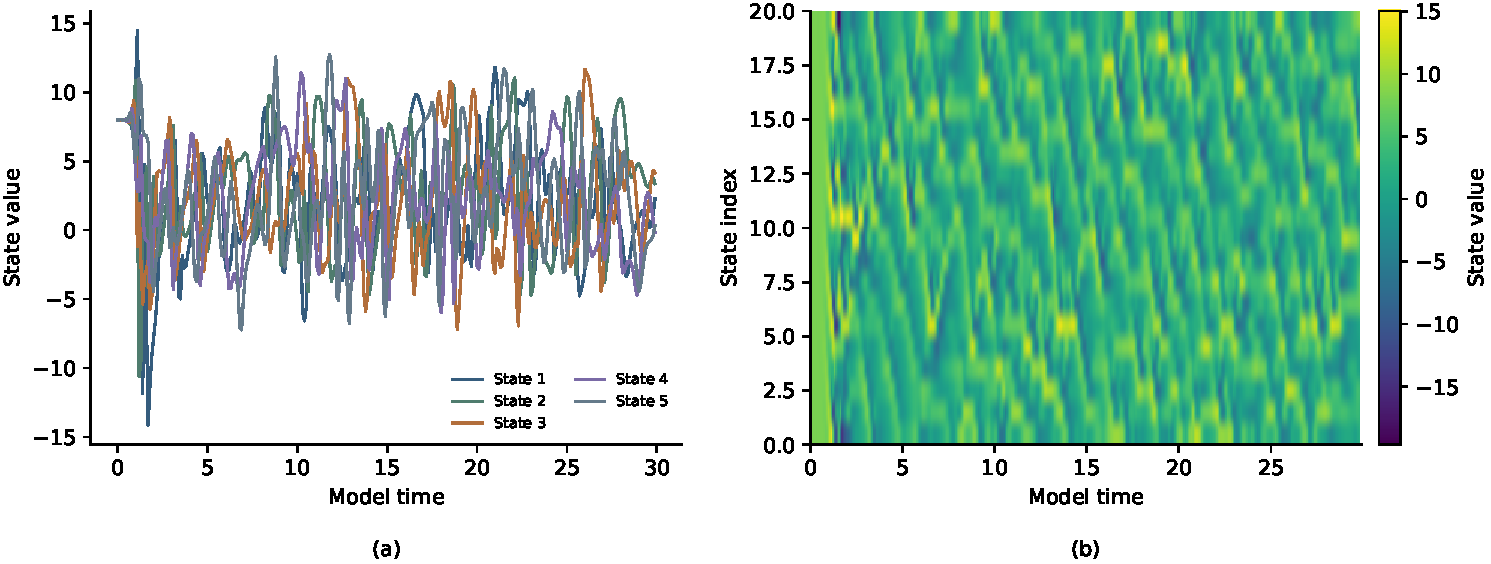
\includegraphics[width=\BookFigureWidth]{figures/ch01_weather_lorenz96.pdf}
\caption{Numerical weather-model surrogate based on the chaotic Lorenz-96 system. (a) Time evolution of five representative state variables under explicit numerical integration. (b) Evolution of all 20 state variables over the same interval; the colorbar reports the state value quantitatively. The simulation illustrates multivariate temporal dependence and rollout sensitivity but is not ERA5 data and is not used to support the published operational benchmark claims in Table~\ref{tab:ch1-weather-benchmark}.}
\label{fig:ch1-weather-lorenz96}
\end{figure}

\begin{table}[t]
\centering
\small
\caption{Published benchmark anchors for data-driven global weather prediction retained from the Pass20 evidence review. Values are meaningful only under their cited data, variables, horizons, and evaluation protocols.}
\label{tab:ch1-weather-benchmark}
\begin{tabular}{p{0.20\textwidth}p{0.24\textwidth}p{0.48\textwidth}}
\toprule
Model / source & Benchmark context & Reported anchor \\
\midrule
GraphCast & 10-day medium-range global forecasting & Reported more accurate than HRES on 90.0\% of 1,380 evaluated targets. \\
Pangu-Weather & ERA5 2018 deterministic forecasts & Reported approximately 10\% lower RMSE than operational IFS and approximately 30\% lower than FourCastNet under the cited protocol. \\
Pangu-Weather & 5-day Z500 example & RMSE 296.7 versus 333.7 for operational IFS and 462.5 for FourCastNet. \\
Pangu-Weather & 24-hour global forecast & Project summary reports approximately 1.4 s inference on an NVIDIA Tesla V100. \\
FourCastNet & IFS comparison & Reported comparable RMSE/ACC to IFS through roughly three days before lagging at longer lead times. \\
WeatherBench 2 & Framework benchmark & Standardized RMSE/ACC comparison environment for AI and numerical weather prediction systems. \\
\bottomrule
\end{tabular}
\end{table}

\textbf{Results}

The numerical surrogate demonstrates why one-step performance cannot characterize a chaotic forecasting system: state trajectories diverge and interact continuously across the rollout. The published benchmark anchors show that modern learned weather models can be competitive with major numerical baselines under carefully specified protocols, but those claims are meaningful only when the data version, variable set, forecast horizon, and evaluation script match.

\textbf{Error Analysis}

Weather-model errors must be stratified by lead time, variable, pressure level, latitude, geographic region, and event type. Aggregate RMSE can hide systematic failures over mountains, coastlines, polar regions, tropical cyclone basins, or rapidly evolving fronts. Spectral diagnostics and conservation-related checks are also useful because a numerically small pointwise error does not guarantee physically realistic spatial structure.

\textbf{Limitations}

Lorenz-96 is a low-dimensional chaotic system and does not reproduce atmospheric dynamics, spherical geometry, moisture processes, radiation, or coupled land-ocean physics. It is used only as a transparent numerical illustration of temporal dependence and rollout sensitivity. The published benchmark table is not a reproduced WeatherBench 2 experiment and should not be read as a homogeneous ranking across unmatched protocols.

\textbf{Deployment / Engineering Implications}

The Chapter 1 lesson is that scientific forecasting credibility depends on validation design. Chronological evaluation, physically appropriate weighting, matched baseline protocols, lead-time analysis, and reproducible data/version control are part of the model assessment itself. A system with strong aggregate RMSE but unstable rollouts or poor extreme-event behavior may still be unsuitable for operational forecasting.
